\documentclass[pdf,ps2pdf,azure,slideColor,colorBG]{prosper}
%\documentclass[pdf,ps2pdf,azure,slideColor,nocolorBG]{prosper}

\usepackage{amssymb}
\usepackage{amsmath}
\usepackage{german}
\usepackage[dvips]{color}
\usepackage{epsfig}
\usepackage{epsf}
\usepackage{graphicx}
%\hypersetup{pdfpagemode=FullScreen}


%%%%%%%%%%%%%% COLOR STUFF %%%%%%%%%%%%%%%%%%%%%%%%%%%%%%%%%%%%%%%%%%%%
% Color to underly headlines, text and footer
% \definecolor{headcolor}{rgb}{0.0, 0.05, 1.0} % used in foilhead
% \definecolor{headcolor}{rgb}{0.15, 0.5, 1.0} % used in foilhead
\definecolor{headcolor}{rgb}{0.30, 0.65, 1.0} % used in foilhead
\definecolor{footcolor}{rgb}{0.2, 0.8, 1.0} % used in page footer
\definecolor{Cboxcolor}{rgb}{1.0, 0.6, 0.6} % used in colored box
\definecolor{Tschwarz}{rgb}{0, 0, 0 }       % from here colors for text
\definecolor{Trot}{rgb}{1.0, 0.0, 0.0}      
\definecolor{Tgruen}{rgb}{0.0, 1.0, 0.0}
% \definecolor{Tblau}{rgb}{0.1, 0.1, 1.0}
\definecolor{Tblau}{rgb}{0.1, 0.3, 1.0}
\definecolor{Tgelb}{rgb}{1.0, 0.9, 0.0}
\newrgbcolor{Cboxrot}{1.0 0.6 0.6}

\newcommand{\headbox}[1]{\fcolorbox{black}{headcolor}{#1}}
\newcommand{\footbox}[1]{\fbox{#1}}
\newcommand{\Cbox}[1]{\colorbox{Cboxcolor}{#1}}
\newcommand{\ROT}[1]{\textcolor{Trot}{#1}}
\newcommand{\GRUEN}[1]{\textcolor{Tgruen}{#1}}
\newcommand{\BLAU}[1]{\textcolor{Tblau}{#1}}
\newcommand{\GELB}[1]{\textcolor{Tgelb}{#1}}



%%% Local Variables: 
%%% mode: latex
%%% TeX-master: t
%%% End: 

\definecolor{weiss}{rgb}{1, 1, 1}
\definecolor{rose}{rgb}{.9, 0.1, 0.1}
\definecolor{schwarz}{rgb}{0, 0, 0 } 
\newcommand{\minos}{\mbox{\red\bf MINOS}}
\newcommand{\cngs}{\mbox{\red\bf CNGS}}
\newcommand{\icarus}{\mbox{\red\bf ICARUS}}
\newcommand{\opera}{\mbox{\red\bf OPERA}}
\newcommand{\jparc}{\mbox{\red\bf T2K}}
\newcommand{\numi}{\mbox{\red\bf NO$\boldsymbol\nu$A}}
\newcommand{\dchooz}{\mbox{\red\bf D-Chooz}}
\newcommand{\RII}{\mbox{\red\bf Reactor-II}}

\newcommand{\mycite}[1] {{\lightgray\tiny #1}}

\newrgbcolor{myred} {1  0.2  0.}

\newcommand{\eVq}  {\text{eV}^2}

\newcommand{\Dmq}    {\Delta m^2}
\newcommand{\BDmq}   {\Delta\overline{m}^2}
\newcommand{\Bnu}    {\overline{\nu}}
\newcommand{\Bsn}    {\overline{s}}
\newcommand{\Bcs}    {\overline{c}}
\newcommand{\Btheta} {\overline{\theta}}


     
%%%%%%%%%%%%%%%%%%%%%%%%%%%%%%%%%%%%%%%%%%%%%%%%%%%%%%%%%%%%%%%%%%%%%%%%%%
%%% command for mathematica import
\newcommand{\Mvariable}[1]{#1}
\newcommand{\Muserfunction}[1]{#1}

%%%%%%%%%%%%%%%%%%%%%%%%%%%%%%%%%%



%-- symbol shorthands and redefinitions -----------------------------

\newcommand{\bea}{\begin{eqnarray*}}
\newcommand{\eea}{\end{eqnarray*}}

\newcommand{\pdagger}{{\phantom{\dagger}}}
\newcommand{\TeV}{\,\mathrm{TeV}}
\newcommand{\GeV}{\,\mathrm{GeV}}
\newcommand{\MeV}{\,\mathrm{MeV}}
\newcommand{\KeV}{\,\mathrm{keV}}
\newcommand{\eV}{\,\mathrm{eV}}
\newcommand{\ecm}{e\,\mathrm{cm}}
\newcommand{\SM}{SU(3)$\times$\protect 
        \linebreak[0]SU(2)$\times$\protect\linebreak[0]U(1)} 
\newcommand{\sm}{{\text{SM}}}
\newcommand{\ord}[1]{\mathcal{O}\left( #1 \right)}
\newcommand{\ordfrac}[2]{\mathcal{O}\fracwithdelims(){#1}{#2}}
\newcommand{\fracwithdelims}[4]{\left#1 \frac{#3}{#4} \right#2}
\newcommand{\vev}[1]{\left\langle #1\right\rangle}
\newcommand{\VeV}[2][]{#1\langle #2 #1\rangle} %% \big\Big\bigg\Bigg  
\newcommand{\interskip}{\medskip}
\newcommand{\Ahalf}[0]{\frac{1}{2}}
\newcommand{\Nup}{{N_{\mu^+}}}
\newcommand{\Num}{{N_{\mu^-}}}
\newcommand{\Nupm}{{N_{\mu^\pm}}}
\newcommand{\nuu}{n_{\mu^-}(\mu^-)}
\newcommand{\nuub}{n_{\mu^+}(\mu^+)}
\newcommand{\neu}{n_{\mu^+}(\mu^-)}
\newcommand{\neub}{n_{\mu^-}(\mu^+)}
\newcommand{\neuvac}{n^{\text{vac}}_{\mu^+}(\mu^-)}
\newcommand{\neubvac}{n^{\text{vac}}_{\mu^-}(\mu^+)}
\newcommand{\eres}{{E_{\text{res}}}}
\newcommand{\nupm}{n^{\text{msw}}_{\nu_\mu}}
\newcommand{\numm}{n^{\text{msw}}_{\bar{\nu}_\mu}}
\newcommand{\reu}{{\nu_e\rightarrow\nu_\mu}}
\newcommand{\rue}{{\nu_{\mu}\rightarrow\nu_e}}
\newcommand{\treu}{{\nu_e\leftrightarrow\nu_\mu}}
\newcommand{\truu}{{\nu_{\mu}\leftrightarrow\nu_\mu}}
\newcommand{\reub}{{\bar{\nu}_e\rightarrow\bar{\nu}_\mu}}
\newcommand{\ruu}{{\nu_\mu\rightarrow\nu_\mu}}
\newcommand{\ruub}{{\bar{\nu}_\mu\rightarrow\bar{\nu}_\mu}}
\newcommand{\rut}{{\nu_\mu\rightarrow\nu_\tau}}
\newcommand{\rutb}{{\bar{\nu}_\mu\rightarrow\bar{\nu}_\tau}}
\newcommand{\ret}{{\nu_e\rightarrow\nu_\tau}}
\newcommand{\retb}{{\bar{\nu}_e\rightarrow\bar{\nu}_\tau}}
\newcommand{\Pee}{P_{\bar\nu_e\rightarrow \bar\nu_e}}
\newcommand{\Pnue}{P_{\nu_\mu\rightarrow \nu_e}}
\newcommand{\emax}{{E_{\text{max}}}}
\newcommand{\emin}{{E_{\text{min}}}}
\newcommand{\NKT}{{N_{\text{kT}}}}
\newcommand{\dm}[1]{{\Delta m^2_{#1}}}
\newcommand{\comment}[1]{(\emph{#1})}
\newcommand{\dms}{\Delta m^2_{21}}
\newcommand{\dma}{\Delta m^2_{31}}
\newcommand{\tho}{\theta_{13}}
\newcommand{\deltacp}{\delta_\textrm{CP}}
\newcommand{\eq}{equation}
\newcommand{\siq}[1]{\sin^2 2 #1}
\newcommand{\si}[1]{\sin 2 #1}
\newcommand{\ie}{{\it i.e.}}
\newcommand{\eg}{{\it e.g.}}
\newcommand{\asf}{{\it a.s.f.}}
\newcommand{\average}[1]{\langle #1 \rangle}
\newcommand{\fig}{figure}

%\newcommand{\ie}{{\it i.e.}}
%\newcommand{\Ie}{{\it I.e.}}
%\newcommand{\eg}{{\it e.g.}}
%\newcommand{\Eg}{{\it E.g.}}
\newcommand{\cf}{{\it cf.}}
\newcommand{\etc}{{\it etc.}}
%\newcommand{\eq}{Equation}
%\newcommand{\eqs}{Equations}
%\newcommand{\Def}{Definition}
%\newcommand{\fig}{figure}
\newcommand{\Fig}{Figure}
\newcommand{\figs}{figures}
\newcommand{\Figs}{Figures}
\newcommand{\Ref}{}
\newcommand{\Refs}{}
\newcommand{\Sec}{section}
\newcommand{\Secs}{sections}
\newcommand{\App}{appendix}
\newcommand{\Apps}{appendices}
\newcommand{\Tab}{table}
\newcommand{\Tabs}{tables}

\newcommand{\rux}{{\nu_\mu\rightarrow\nu_x}}
\newcommand{\ruxb}{{\bar{\nu}_\mu\rightarrow\bar{\nu}_x}}
%\newcommand{\ruxb}{{\bar{\nu}_\mu\rightarrow\bar{\nu}_x}}
%\newcommand{\ruub}{{\bar{\nu}_\mu\rightarrow\bar{\nu}_\mu}}
\newcommand{\reeb}{{\bar{\nu}_e\rightarrow\bar{\nu}_e}}
\newcommand{\ree}{{\nu_e\rightarrow\nu_e}}
%\newcommand{\rut}{{\nu_\mu\rightarrow\nu_\tau}}
%\newcommand{\rutb}{{\bar{\nu}_\mu\rightarrow\bar{\nu}_\tau}}
%\newcommand{\ret}{{\nu_e\rightarrow\nu_\tau}}
%\newcommand{\retb}{{\bar{\nu}_e\rightarrow\bar{\nu}_\tau}}
\newcommand{\dchi}{\Delta\chi^2}

\newcommand{\pc}[1]{\chi^2_{#1}}
\newcommand{\tli}{\pc{\text{\sc l}}}
\newcommand{\hie}{\pc{\text{\sc h}}}
\newcommand{\acp}{\pc{\text{\sc cp}}}
\newcommand{\acpv}{\acp}
\newcommand{\mcpv}{\acp(\pm)}
%%%%%%%%%%%%%%%%%%%%%%%%%%%%%%%%%%%%%%%%%%%%%%%%%%%%%%%%%%%%%%%%
%%%%%%%%%%%%%%%% Our beautiful setups ;-) %%%%%%%%%%%%%%%%%%%%%%
%%%%%%%%%%%%%%%%%%%%%%%%%%%%%%%%%%%%%%%%%%%%%%%%%%%%%%%%%%%%%%%%
%\newcommand{\numi}{{\sf NuMI}}
\newcommand{\nfII}{{\sf NuFact-II}}
\newcommand{\nfI}{{\sf NuFact-I}}
\newcommand{\jsk}{{\sf JHF-SK}}
\newcommand{\jhk}{{\sf JHF-HK}}
\newcommand{\rI}{{\sf Reactor-I}}
\newcommand{\rII}{{\sf Reactor-II}}
\newcommand{\lmai}{{\sc lma-i}}
\newcommand{\lmaii}{{\sc lma-ii}}
\newcommand{\JHFHK}{{\sf JHF-HK}}
\newcommand{\JHFSK}{{\sf JHF-SK}}
\newcommand{\NuFactI}{{\sf NuFact-I}}
\newcommand{\NuFactII}{{\sf NuFact-II}}
\newcommand{\sigI}{$68.27\%$}
\newcommand{\sigII}{$95.45\%$}
\newcommand{\sigIII}{$99.73\%$}
\newcommand{\cpv}{{\sc cp}-violation}
\newcommand{\cpc}{{\sc cp}-conservation}
\newcommand{\dof}{{\sc dof}}
\newcommand{\lmaI}{{\sc lma-i}}
\newcommand{\lmaII}{{\sc lma-ii}}
\newcommand{\tgwy}{\mathrm{t}\,\mathrm{GW}\,\mathrm{y}}

%%%%%%%%%%%%%%%%%%%%%%%%%%%%%%%%%%%%%%%%%%%%%%%%%%%%%%%%%%%%%%%%

%%%%%%%%%%%%%%%%%%%%%%%%%%%%%%%%%%%%%%%%%%%%%%%%%%%%%%%%%%%%
%%%%%%%%%%% Meine privaten Kommandos %%%%%%%%%%%%%%%%%%%%%%%
%%%%%%%%%%%%%%%%%%%%%%%%%%%%%%%%%%%%%%%%%%%%%%%%%%%%%%%%%%%%
\newcommand{\nuf}{Neutrino-Fabrik}
\newcommand{\unit}[2]{$ #1\thinspace\mbox{{\rm #2}}$}
\newcommand{\nee}{n_{\mu^+}(e^-)}
\newcommand{\neeb}{n_{\mu^-}(e^+)}
\newcommand{\abrev}[2]{{\sc #1}{\it #2}}
\newcommand{\abr}[1]{{\sc\lowercase{#1}}}
\newcommand{\rcite}[1]{\/{\rm \cite{#1}}}
\newcommand{\szt}[1]{\sin^22\theta_{#1}}
\newcommand{\decf}[1]{{\rm [\abr{nfb}\thinspace$\rightarrow$\thinspace\abr{#1}]}} 
\newcommand{\decw}[1]{{\rm
    [\abr{WBB}\thinspace$\rightarrow$\thinspace\abr{#1}]}} 
\newcommand{\ver}[1]{{\sf #1}}
\newcommand{\cpp}{{{\sc cp}-phase}}
\newcommand{\app}{appendix}
\newcommand{\chap}{chapter}
\newcommand{\sct}{section}
\newcommand{\bs}[1]{\boldsymbol{#1}}
\newcommand{\cl}{{\sf cl}}
\newcommand{\rb}[1]{\raisebox{1.5ex}[-1.5ex]{#1}}

%%%%%%%%%%%%%%%%%%%%%%%%%%%%%%%%%%%%%%%%%%%%%%%%%%%%%%

\title{Software Tools}


\author{Patrick Huber}
\institution{University of Wisconsin -- Madison\\[4ex]
{\small ~\\[9ex]
International Neutrino Factory and Superbeam Scoping Study\\
CERN\\
 22-24 September 2005

}}
\slideCaption{P. Huber}
%%%%%%%%%%%%%%%%%%%%%%%%%%%%%%%%%%%%%%%%%%%%%%%%%%%%%%
\begin{document}

\maketitle

%%%%%%%%%%%%%%%%%%%%%%%%%%%%%%%%%%%%%%%%%%%%%%%%%%%%%%
\overlays{1}{
  \begin{slide}{Outline}
    \begin{itemize}
    \item General HEP software
    \item Requirements for the physics group
    \item GLoBES 
      \begin{itemize}
      \item[\GRUEN{-}] Features
\item[\GRUEN{-}] Structure
\item[\GRUEN{-}] C-API
\item[\GRUEN{-}] AEDL
\end{itemize}
\item Summary
\end{itemize}
\end{slide}}

%%%%%%%%%%%%%%%%%%%%%%%%%%%%%%%%%%%%%%%%%%%%%%%%%%%%%
\begin{slide}{General HEP Software}
\begin{itemize}
\item ROOT
\item GEANT
\item NUANCE --\\
 neutrino event generator by Dave Casper
\end{itemize}

These tools are especially important for the detector and accelerator
working groups.\\

\end{slide}


%%%%%%%%%%%%%%%%%%%%%%%%%%%%%%%%%%%%%%%%%%%%%%%%%%%%%%

\begin{slide}{General Requirements}

Simulation
\begin{itemize}
\item fast pseudo-Monte-Carlo 
\item Efficiencies
\item Backgrounds
\item Energy response 
\end{itemize}
Interface to the detector/accelerator working groups
\end{slide}

%%%%%%%%%%%%%%%%%%%%%%%%%%%%%%%%%%%%%%%%%%%%%%%%%%%%%%

\begin{slide}{General Requirements}
Analysis
\begin{itemize}
\item Appearance channels
\item Disappearance channels
\item Energy information
\item External information 
\end{itemize}

\begin{itemize}
\item Systematics
\item Correlations
\item Matter density uncertainties
\item Degeneracies
\end{itemize}


\end{slide}
%%%%%%%%%%%%%%%%%%%%%%%%%%%%%%%%%%%%%%%%%%%%%%%%%%%%%%%%
\begin{slide}{General Requirements}


Comparison
\begin{itemize}
\item Parameters of interest
\item Figure(s) of merit
\item Risk function
\end{itemize}


\end{slide}


%%%%%%%%%%%%%%%%%%%%%%%%%%%%%%%%%%%%%%%%%%%%%%%%%%%%%%
\begin{slide}{}

\begin{minipage}{12.5cm}
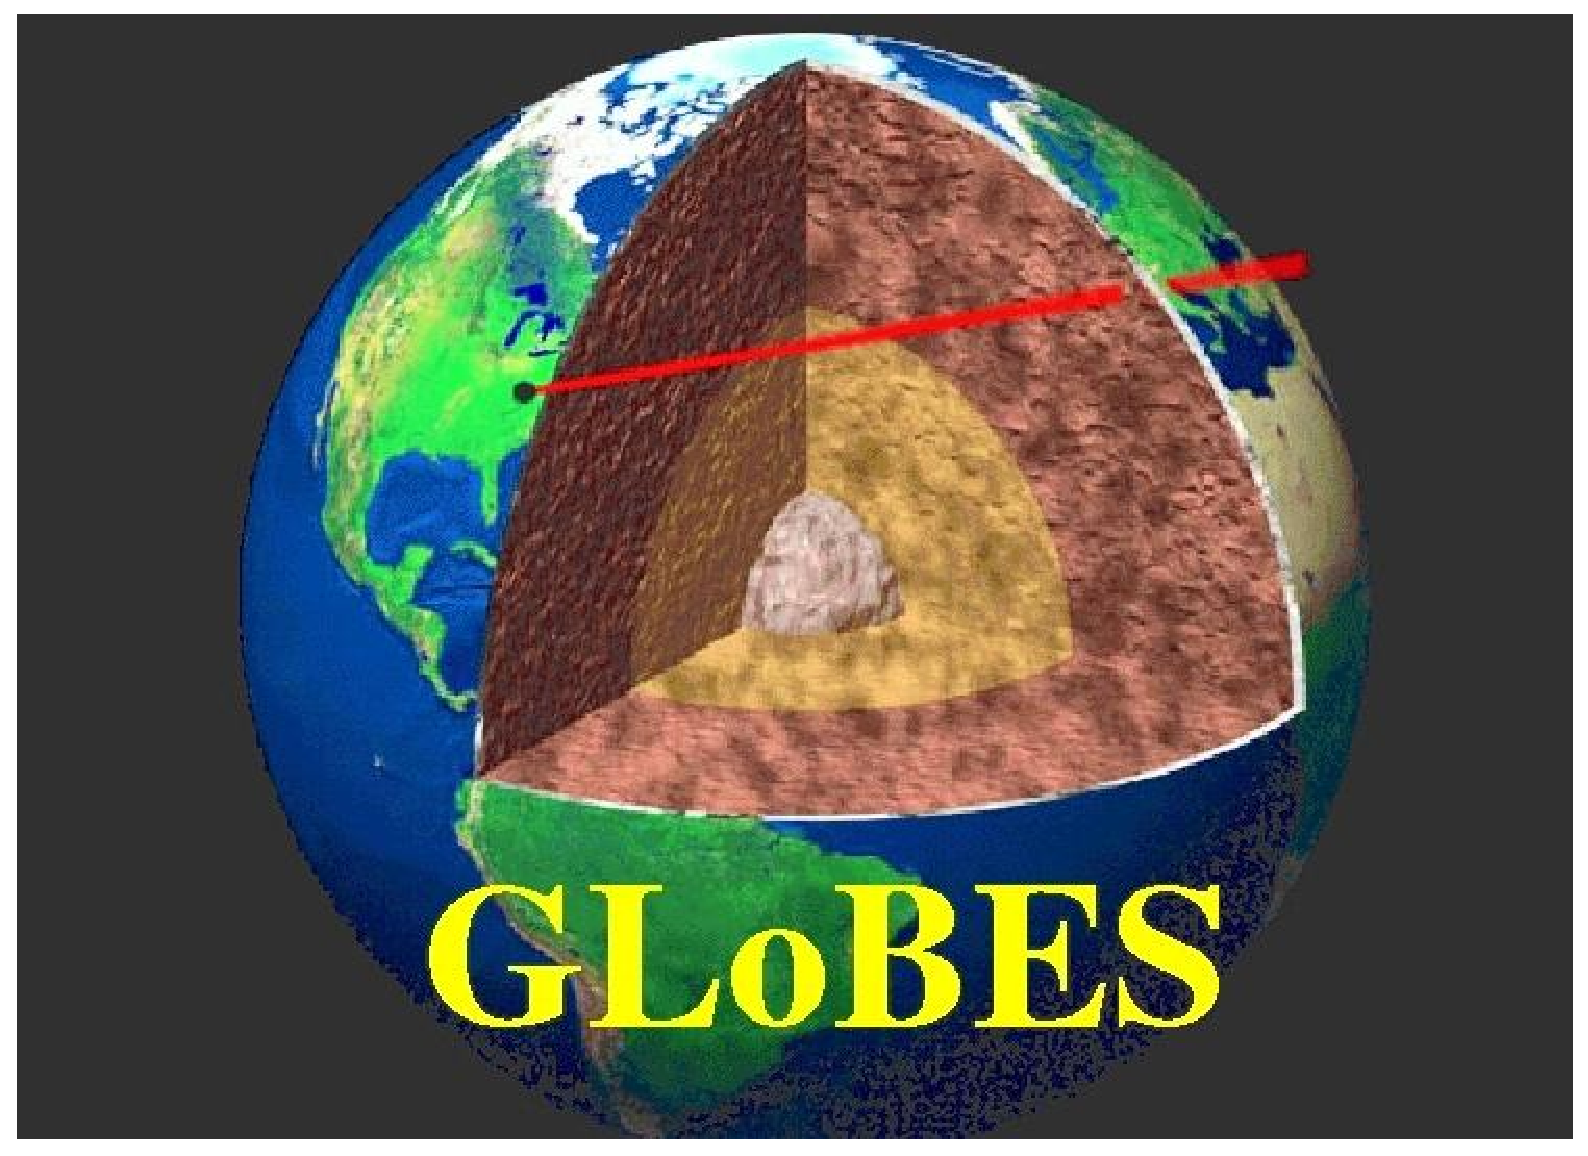
\includegraphics[angle=0,width=10cm]{globes}
\end{minipage}
\end{slide}
%%%%%%%%%%%%%%%%%%%%%%%%%%%%%%%%%%%%%%%%%%%%%%%%%%%%
\begin{slide}{}
\vspace*{1cm}

{\Large General Long Baseline\\ Experiment Simulator}\\[1cm]

GLoBES is a software package designed for 
\begin{itemize}
\item Simulation
\item Analysis
\item Comparison
\end{itemize}
of neutrino oscillation experiments

\end{slide}
%%%%%%%%%%%%%%%%%%%%%%%%%%%%%%%%%%%%%%%%%%%%%%%%%%%%%%
\begin{slide}{Why use GLoBES?}

\begin{itemize}
\item Avoids re-inventing the wheel
\item Well defined interface between beam, detector and neutrino
  physics
\item Facilitates data exchange
\item Encourages collaboration
\item Easy comparison of different setups

\end{itemize}
\end{slide}


%%%%%%%%%%%%%%%%%%%%%%%%%%%%%%%%%%%%%%%%%%%%%%%%%%%%%%
\begin{slide}{GLoBES -- features}

\begin{itemize}
\item Accurate treatment of systematical errors
\item Arbitrary matter profile \& uncertainties
\item Arbitrary energy resolution function
\item Single and multiple experiment simulation
\item Simple $\chi^2$ calculation
\item Inclusion of external input
\item Projection of $\chi^2$ (minimization)
\item ...
\end{itemize}
\end{slide}

%%%%%%%%%%%%%%%%%%%%%%%%%%%%%%%%%%%%%%%%%%%%%%%%%%%%%%
\begin{slide}{GLoBES -- features}

Example -- $\chi^2$ projections\\
\fcolorbox{schwarz}{weiss}{
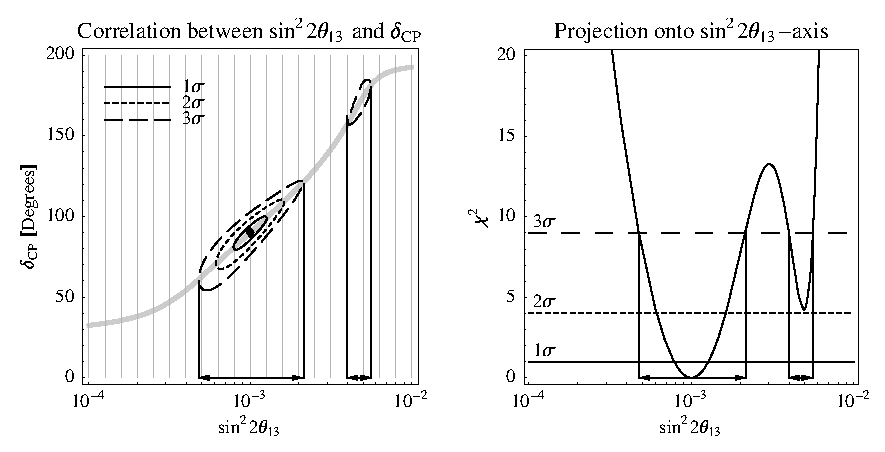
\includegraphics[width=10cm]{projex}
}
{\tiny figure taken from PH, M. Lindner, W. Winter, Comput.\ Phys.\ Commun.\  {\bf 167} (2005) 195}

\end{slide}
%%%%%%%%%%%%%%%%%%%%%%%%%%%%%%%%%%%%%%%%%%%%%%
\begin{slide}{GLoBES -- features}

GLoBES has been used for simulating
\begin{itemize}
\item MINOS, CNGS
\item Reactor experiments, Double-CHOOZ
\item T2K
\item NO$\nu$A
\item JHF-HK (T2K upgrade)
\item Neutrino factory
\item $\beta$-beam
\item BNL neutrino beam
\end{itemize}
\end{slide}
%%%%%%%%%%%%%%%%%%%%%%%%%%%%%%%%%%%%%%%%%%%%%
\begin{slide}{The GLoBES-Team}

GLoBES is developed, documented, maintained and supported by
\begin{itemize}
\item Patrick Huber (UW)
\item Joachim Kopp (TUM)
\item Manfred Lindner (TUM)
\item Mark Rolinec (TUM)
\item Walter Winter (IAS)
\end{itemize}
\vspace*{1cm}
The GLoBES tar-ball as well as an extensive manual 
are available since August 2004 at\\
\begin{center}
{\tt http://www.ph.tum.de/$\,\tilde{}$globes/}
\end{center} 

\end{slide}


%%%%%%%%%%%%%%%%%%%%%%%%%%%%%%%%%%%%%%%%%%%%%%%%%%%%%%
\begin{slide}{GLoBES -- basic structure}

\fcolorbox{schwarz}{weiss}{
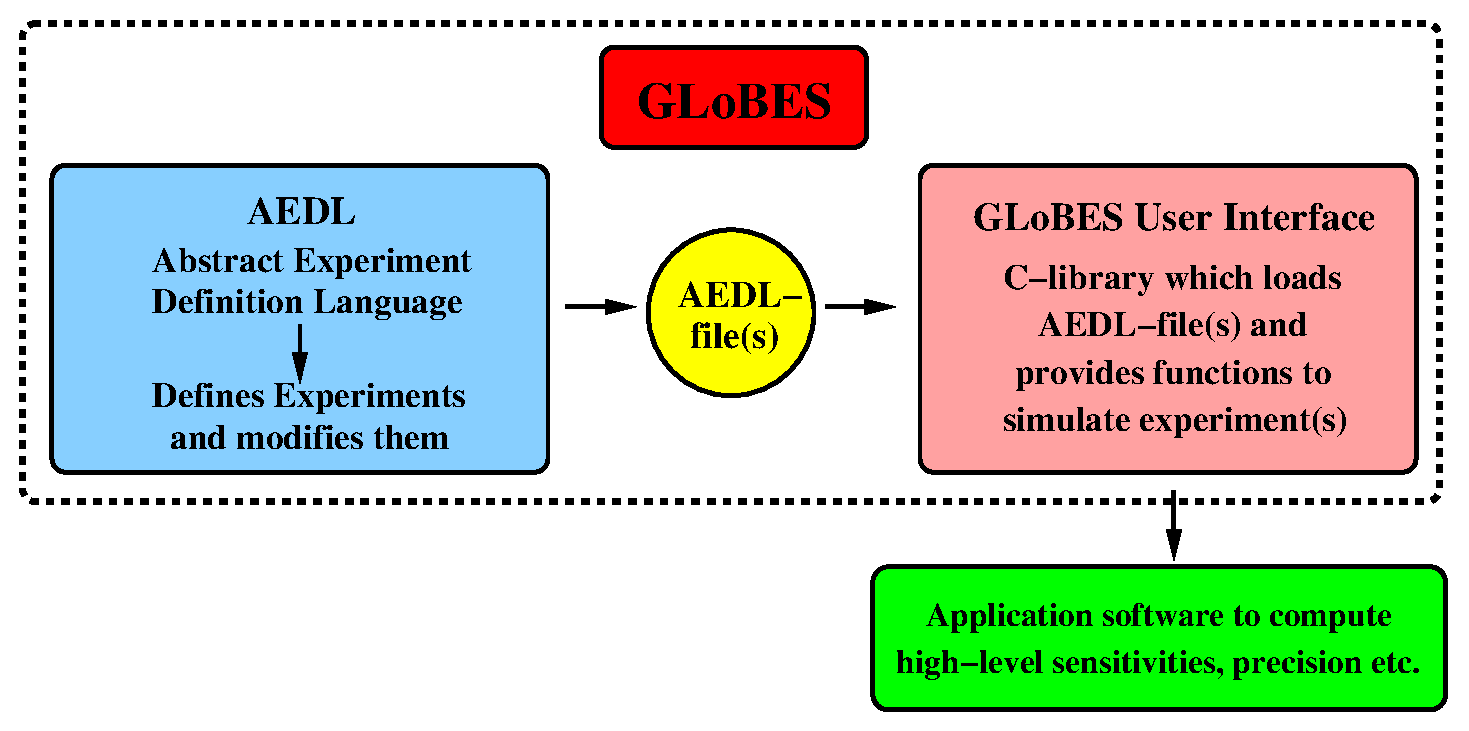
\includegraphics[width=11cm]{GLOBES}
}
{\tiny figure taken from PH, M. Lindner, W. Winter, Comput.\ Phys.\ Commun.\  {\bf 167} (2005) 195}

\end{slide}


%%%%%%%%%%%%%%%%%%%%%%%%%%%%%%%%%%%%%%%%%%%%%%%%%%%%%%
\overlays{3}{\begin{slide}{GLoBES -- C API}
\onlySlide*{1}{
How do you this ?\\
\fcolorbox{schwarz}{weiss}{
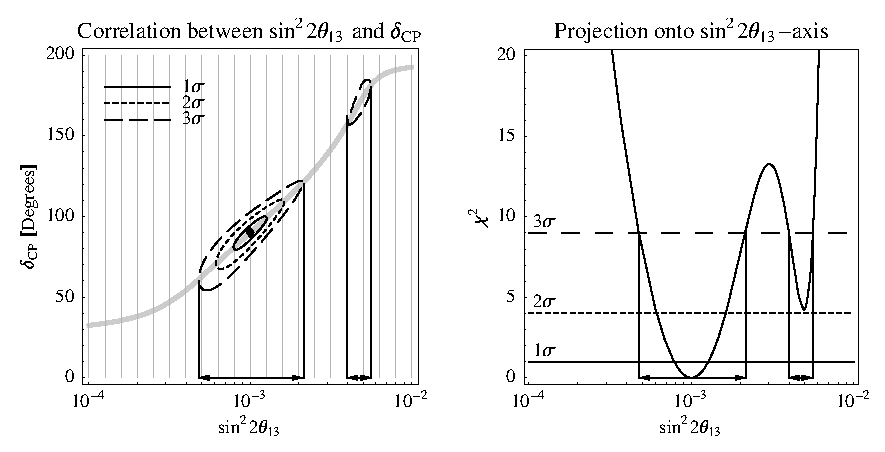
\includegraphics[width=10cm]{projex}
}}

\onlySlide*{2}{
\hspace{-1cm}\fcolorbox{schwarz}{weiss}{
\begin{minipage}{12cm}
{\tt {\tiny
  /* Set starting values and input errors for all projections */  \\
  glbDefineParams(input\_errors,theta12*0.1,0,0,0,sdm*0.1,0);\\  
  glbSetDensityParams(input\_errors,0.05,GLB\_ALL);\\
  glbSetStartingValues(true\_values);\\
  glbSetInputErrors(input\_errors);\\
~\\
  /* Define my own two-parameter projection for glbChiNP: Only deltacp is free! */ \\
  glbDefineProjection(th13\_projection,GLB\_FIXED,GLB\_FIXED,GLB\_FIXED,\\
\hspace*{19ex}GLB\_FREE,GLB\_FIXED,GLB\_FIXED); \\
  glbSetProjection(th13\_projection); 
}}
\end{minipage}
}}
\onlySlide*{3}{
\hspace{-1cm}\fcolorbox{schwarz}{weiss}{
\begin{minipage}{12cm}
{\tt {\tiny
  /* Iteration over all values to be computed */ \\
  double x,res1,res2;     \\
  for(x=-4;x<-2.0+0.001;x=x+2.0/50) \\
  \{ \\
  /* Set fit value of stheta */ \\
 glbSetOscParams(test\_values,asin(sqrt(pow(10,x)))/2,1); \\
   
 /* Guess fit value for deltacp in order to safely find minimum */ \\
 glbSetOscParams(test\_values,200.0/2*(x+4)*M\_PI/180,3); \\
 
 /* Compute Chi2 for user-defined two-parameter correlation */ \\
 res1=glbChiNP(test\_values,NULL,GLB\_ALL); \\
     
 /* Compute Chi2 for full correlation: minimize over all but theta13 */ \\
 res2=glbChiTheta(test\_values,NULL,GLB\_ALL); \\
 
 AddToOutput(x,res1,res2);\\
  \}   
}}
\end{minipage}
}}
\end{slide}}
%%%%%%%%%%%%%%%%%%%%%%%%%%%%%%%%%%%%%%%%%%%%%%%%%%%%%%
\overlays{2}{\begin{slide}{GLoBES -- AEDL}
\onlySlide*{1}{\fcolorbox{schwarz}{weiss}{
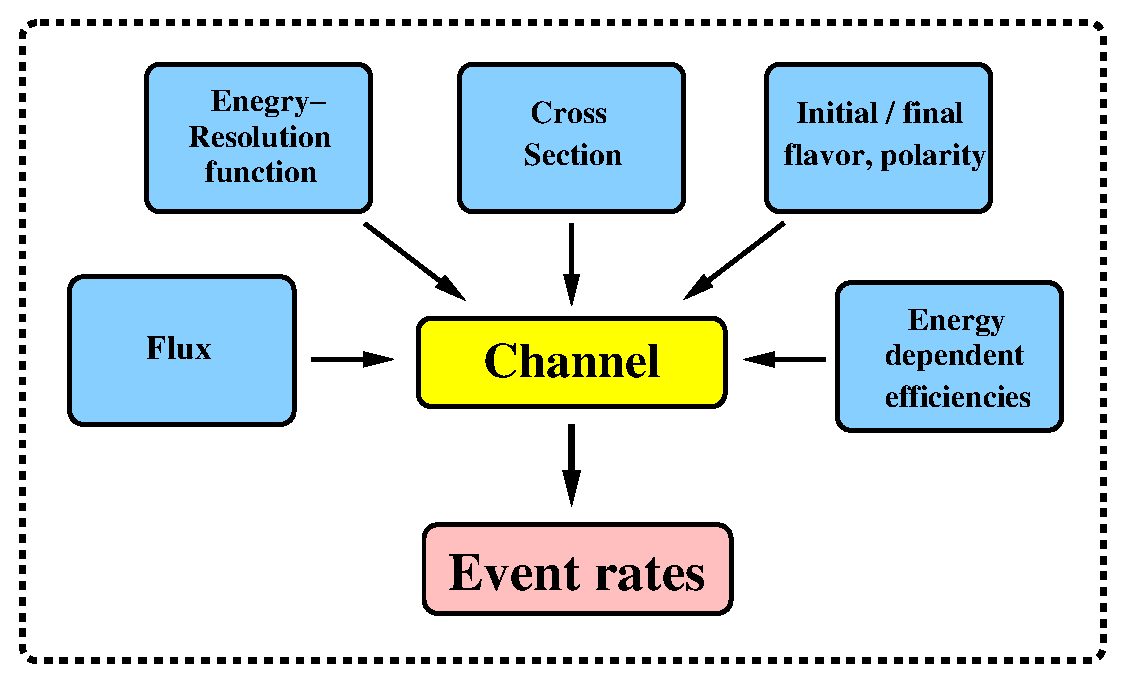
\includegraphics[width=10cm]{AEDL1}
}
~\\{\tiny figure taken from PH, M. Lindner, W. Winter, Comput.\ Phys.\ Commun.\  {\bf 167} (2005) 195}
}
\onlySlide*{2}{
Neutrino factory example\\
~\hspace{-1cm}\fcolorbox{schwarz}{weiss}{
\begin{minipage}{12cm}
{\tt {\tiny
  channel(\#mu\_minus\_appearance)<\\
\hspace*{1cm}@channel =      \#mu\_plus:   +:      e:      m:      \#CC:    \#sm0\\
\hspace*{1cm}@post\_smearing\_efficiencies = \{0.07, 0.21, 0.35, 0.50,
        0.65, 0.80,\\
\hspace*{2cm} 0.93, 1, 1,1, 1, 1, 1, 1,1, 1, 1, 1, 1, 1\}\\
>   
}}
\end{minipage}
}

}
\end{slide}}
%%%%%%%%%%%%%%%%%%%%%%%%%%%%%%%%%%%%%%%%%%%%%%%%%%%%%%
\overlays{2}{\begin{slide}{GLoBES -- AEDL}
\onlySlide*{1}{\fcolorbox{schwarz}{weiss}{
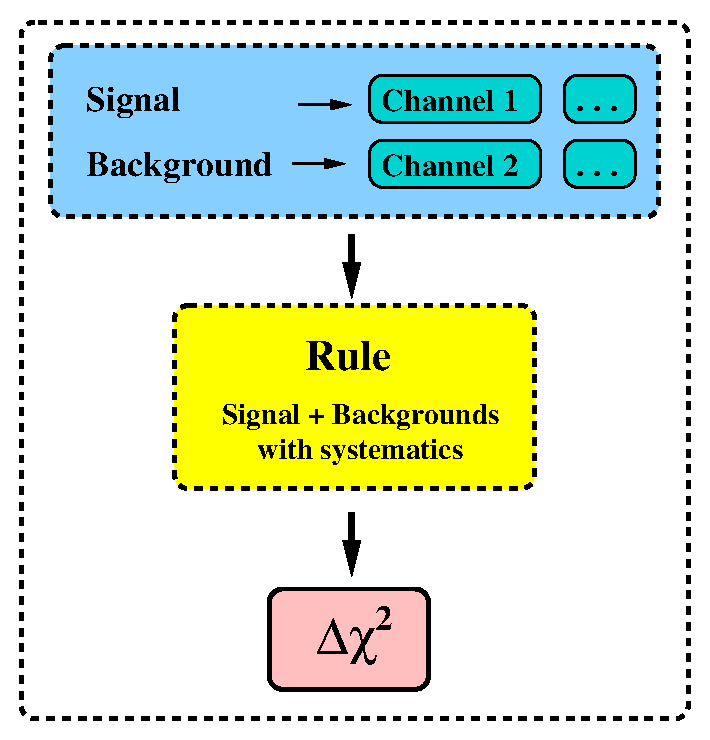
\includegraphics[width=7cm]{SignalBackground}
}
~\\{\tiny figure taken from PH, M. Lindner, W. Winter, Comput.\ Phys.\ Commun.\  {\bf 167} (2005) 195}
}
\onlySlide*{2}{
Neutrino factory example\\
~\hspace{-1cm}\fcolorbox{schwarz}{weiss}{
\begin{minipage}{12cm}
{\tt {\tiny
  rule(\#wrong\_sign\_muons\_1)<\\
~\\
\hspace*{1cm}        @signal =             0.45@\#mu\_minus\_appearance\\
\hspace*{1cm}        @signalerror =       0.001  :       0.0001\\
~\\
\hspace*{1cm}        @background =            1@\#mu\_plus\_disappearance\\
\hspace*{1cm}        @backgrounderror =           2e-06  :       0.0001\\
\hspace*{1cm}        @backgroundcenter =          1e-05  :            0\\
~\\
\hspace*{1cm}        @errordim\_sys\_on =      0\\
\hspace*{1cm}        @errordim\_sys\_off =     2\\
\hspace*{1cm}        @energy\_window =                 4  :           50\\
~\\
>

}}
\end{minipage}
}

}


\end{slide}}


%%%%%%%%%%%%%%%%%%%%%%%%%%%%%%%%%%%%%%%%%%%%%%%%%%%%%%
\begin{slide}{GLoBES -- AEDL}
\fcolorbox{schwarz}{weiss}{
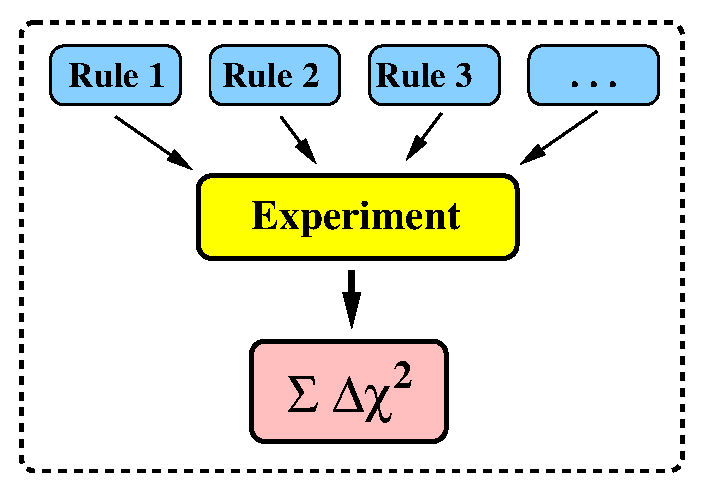
\includegraphics[width=10cm]{Rules}
}
~\\
{\tiny figure taken from PH, M. Lindner, W. Winter, Comput.\ Phys.\ Commun.\  {\bf 167} (2005) 195}
\end{slide}

%%%%%%%%%%%%%%%%%%%%%%%%%%%%%%%%%%%%%%%%%%%%%%%%%%%%%%%%%%%%%%%%%%%%%%
%                summary                                             %
%%%%%%%%%%%%%%%%%%%%%%%%%%%%%%%%%%%%%%%%%%%%%%%%%%%%%%%%%%%%%%%%%%%%%%

%---------------------------------------------------------------------- SLIDE -
\overlays{1}{
\begin{slide}{Summary}
GLoBES is a
\begin{itemize}
\item a well tested
\item powerful
\item flexible
\end{itemize}
software package for the
\begin{itemize}
\item Simulation
\item Analysis
\item Comparison
\end{itemize}
of neutrino oscillation experiments
\end{slide}
}


%%%%%%%%%%%%%%%%%%%%%%%%%%%%%%%%%%%%%%%%%%%%%%%%%%%%%%

%%%%%%%%%%%%%%%%%%%%%%%%%%%%%%%%%%%%%%%%%%%%%%%%%%%%%%
\end{document}





%%%%%%%%%%%%%%%%%%%%%%%%%%%%%%%%%%%%%%%%%%%%%%%%%%%%%%
\begin{slide}{GLoBES -- features}
\fcolorbox{schwarz}{weiss}{
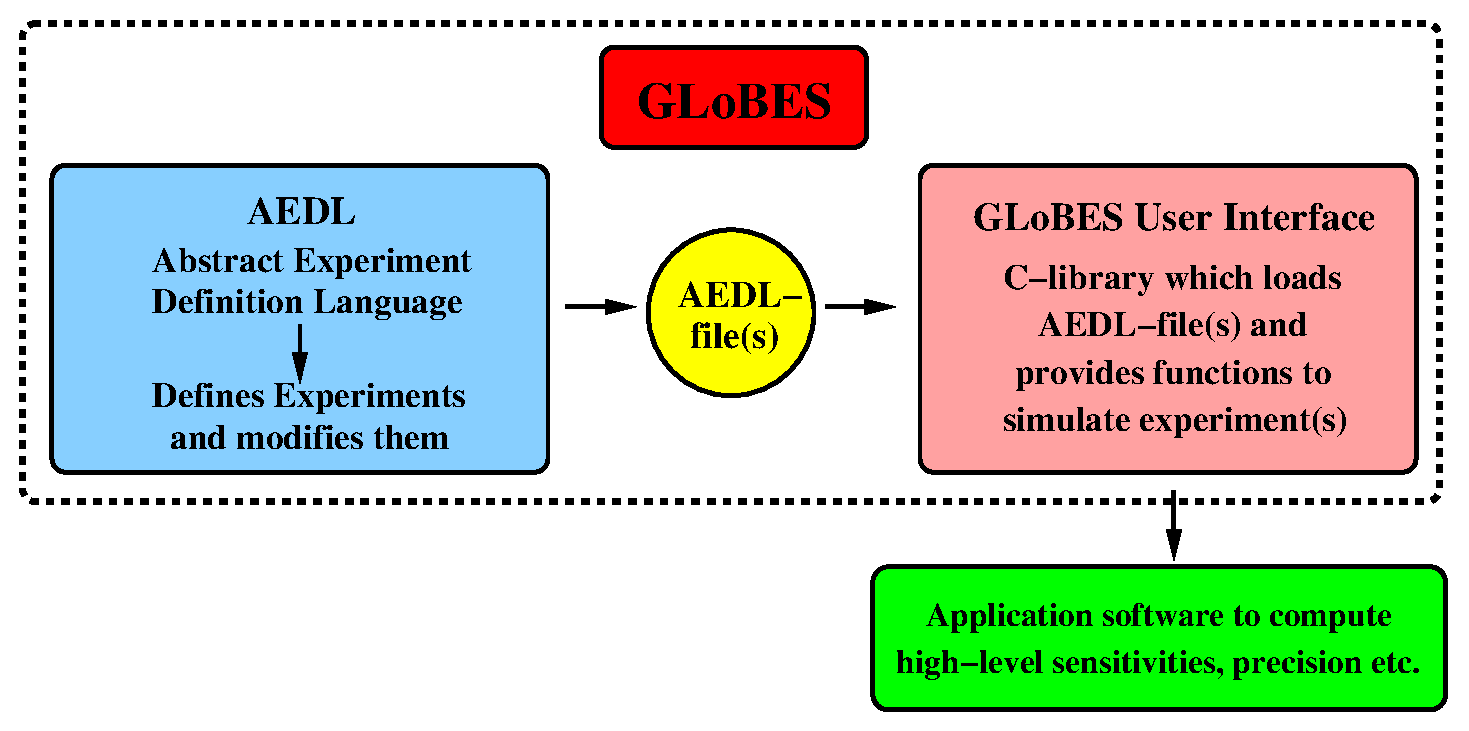
\includegraphics[width=10cm]{GLOBES}
}
\end{slide}

%%%%%%%%%%%%%%%%%%%%%%%%%%%%%%%%%%%%%%%%%%%%%%%%%%%%%%
\overlays{1}{\begin{slide}{GLoBES -- AEDL}
\onlySlide*{1}{\fcolorbox{schwarz}{weiss}{
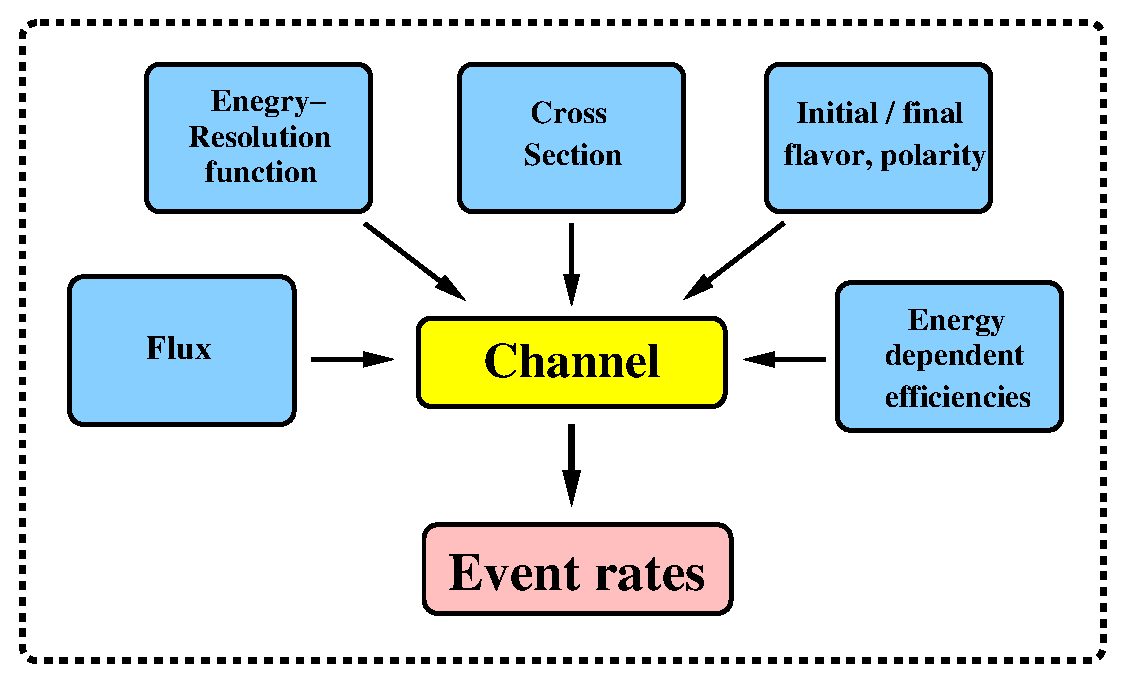
\includegraphics[width=10cm]{AEDL1}
}}
\end{slide}}
%%%%%%%%%%%%%%%%%%%%%%%%%%%%%%%%%%%%%%%%%%%%%%%%%%%%%%
\overlays{1}{\begin{slide}{GLoBES -- AEDL}
\onlySlide*{1}{\fcolorbox{schwarz}{weiss}{
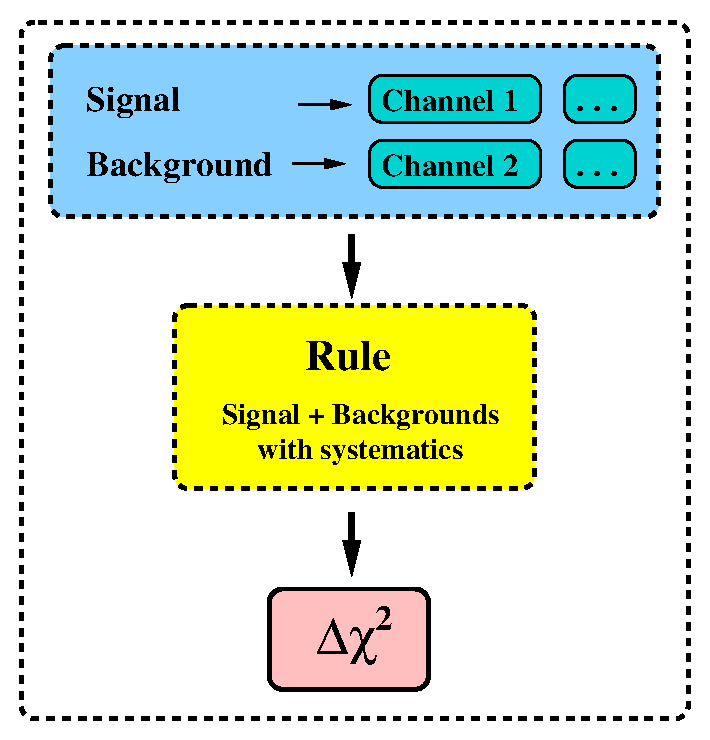
\includegraphics[width=7cm]{SignalBackground}
}}

\end{slide}}
%%%%%%%%%%%%%%%%%%%%%%%%%%%%%%%%%%%%%%%%%%%%%%%%%%%%%%
\begin{slide}{GLoBES -- AEDL}
\fcolorbox{schwarz}{weiss}{
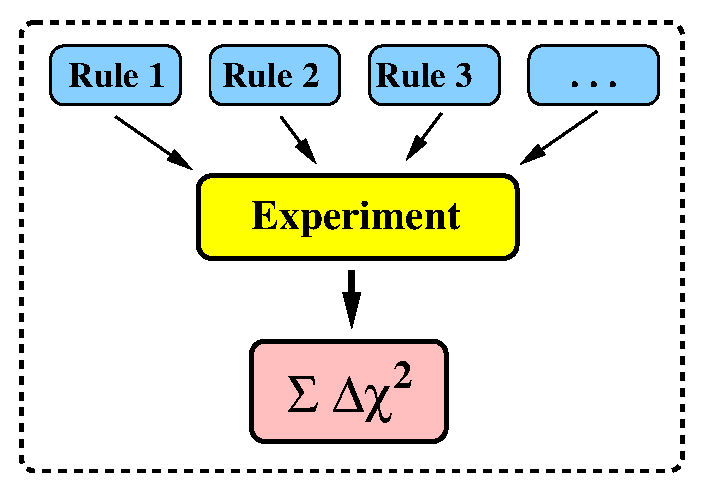
\includegraphics[width=10cm]{Rules}
}
\end{slide}




